\documentclass[aspectratio=169]{beamer}
\setbeamertemplate{navigation symbols}{}
\usepackage{color,amsmath,comment, subfigure}
\usepackage{booktabs}
\usepackage{url}


%%%%%%%%%%%%%%%%%%%%%%%%%%
\title[]{Class 13: Respondent-driven sampling}
\author[]{Matthew J. Salganik}
\institute[]{Sociology 204: Social Networks\\Princeton University}
\date[]{
1/3 Background and data collection
\vfill
\begin{flushleft}
\vspace{0.6in}
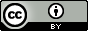
\includegraphics[width=0.1\textwidth]{figures/cc.png}
\end{flushleft}

}

\begin{document}
%%%%%%%%%%%%%%%%%%%%%%%%%%%
\frame{\titlepage}
%%%%%%%%%%%%%%%%%%%%%%%%%%%
\section{Introduction}
%%%%%%%%%%%%%%%%%%%%%%%%%%%
\begin{frame}
\frametitle{Introduction}
There are an estimated 38 million people [31.6 million–44.5 million] living with HIV in 2019.  In most countries, the disease is concentrated in three high risk groups:
\begin{itemize}
\item drug users 
\item commercial sex workers
\item men who have sex with men 
\end{itemize}
\vfill
Better information about these group can be used to understand and control the spread of HIV/AIDS: ``know your epidemic''
\end{frame}
%%%%%%%%%%%%%%%%%%%%%%%%%%%
\frame{
\frametitle{Hidden populations}
These ``hidden'' populations are hard to sample because:
\begin{itemize}
\item No sampling frame
\item Small proportion of the general population
\item In some cases, desire to remain anonymous
\end{itemize}
}
%%%%%%%%%%%%%%%%%%%%%%%%%%%
\frame{
\frametitle{Previous approaches to the study of hidden populations}
\textcolor{blue}{Institutional sampling}: Samples drug injectors in treatment.\\
\pause
\vfill
Relatively inexpensive, but difficult to generalize from institutionalized population to the non-institutionalized population.
}
%%%%%%%%%%%%%%%%%%%%%%%%%%%
\frame{
\frametitle{Previous approaches to the study of hidden populations}
\textcolor{blue}{Targeted sampling}  (Watters and Biernacki, 1989): Through a combination of methods, accesses populations members outside of institutional settings.\\
\vfill
\pause
Despite wider coverage, it is not possible clear how to the hidden population because probability of selection is not known.
}
%%%%%%%%%%%%%%%%%%%%%%%%%%%
\frame{
\frametitle{Previous approaches to the study of hidden populations}
\textcolor{blue}{Time-location sampling}: Construct sampling frame of time/locations, \pause but 
\begin{itemize}
\item Data collection is expensive and time consuming
\pause
\item Requires adjustments for oversampling people who frequently attend elements on sampling frame
\pause
\item Not all time/location combinations are accessible to researchers 
\end{itemize}
\vfill
In some cases, it may not be possible to generalize to the hidden population.  For example, drug injectors who attend venues accessible to researchers may be different from those who don't.\\
}
%%%%%%%%%%%%%%%%%%%%%%%%%%%
\frame{
\frametitle{Another approach: snowball sampling}
Instead of thinking of people as atomized units on a sampling frame, think of people as \textcolor{blue}{embedded in networks}.  Friends recruit friends and the sample progresses through the social network.  But, conventional wisdom was that it was not possible to make unbiased estimates from \textcolor{blue}{snowball samples} because they:
\begin{itemize}
\item oversample popular people
\item non-independence of observations (people are similar to their friends)
\item depended on the choice of seeds
\end{itemize}
}
%%%%%%%%%%%%%%%%%%%%%%%%%%%
\frame{
\frametitle{Respondent-driven sampling}
It turns out that unbiased estimation is possible \textcolor{blue}{under certain conditions} (Salganik and Heckathorn, 2004), and the process is cheaper and faster than existing methods.  Respondent-driven sampling is now being used by many researchers: \pause
\begin{itemize}
\item More than 100 studies studies in 29 countries involving more then 30,000 respondents (Malekinejad, et al, 2007) \pause
\item Drug injector portion of the U.S. Center for Disease Control (CDC) National HIV Behavioral Surveillance System,  repeated cross-sectional study in 25 largest U.S. cities (samples of 500 in each city)
\end{itemize}
}
%%%%%%%%%%%%%%%%%%%%%%%%%%%
\begin{frame}

Respondent-driven sampling describes both:
\begin{itemize}
\item a method of data collection
\item a method of estimation
\end{itemize}

\end{frame}
%%%%%%%%%%%%%%%%%%%%%%%%%%%
\begin{frame}
\frametitle{Sampling}

Sample progresses using \textcolor{blue}{dual-incentive system} (respondents are paid to participant and to recruit others).  Participants come to store-front location with coupon (Heckathorn 1997).\\
\begin{center}
\includegraphics<1>[width=0.4\textwidth]{figures/coupon}
\end{center}
\pause
Two additional steps:
\begin{itemize}
\item non-duplication
\pause
\item population verification
\end{itemize}

\end{frame}
%%%%%%%%%%%%%%%%%%%%%%%%%%%
\frame{
\frametitle{Sampling}
\begin{center}
\includegraphics<1>[width=0.5\textwidth]{figures/nyc-idus}
\end{center}
Recruitment network from a study of drug users in New York City (Abdul-Quader et al., 2006)
\begin{itemize}
\item 8 seeds $\rightarrow$ 618 drug users
\item 13 weeks
\end{itemize}
}
%%%%%%%%%%%%%%%%%%%%%%%%%%%
\frame{
\frametitle{Reach of the sampling method}
RDS as a sampling methods seems to work very well in a range of contexts \pause
\begin{itemize}
\item It has been able to reach populations that the researchers had trouble accessing: men who have sex with men in Kampala, Uganda (Kajubi et al. 2007) 
\pause
\item Seems to work better for drug injectors than sex workers
\pause
\item Even if there are problems with statistical inference, still provides access to the population (McFarland)
\end{itemize}
}
%%%%%%%%%%%%%%%%%%%%%%%%%%%
\begin{frame}

But, this sample is not a simple random sample.  In the next video we will learn how to make estimates from this kind of data.

\end{frame}

\end{document}
